\newpage
\section{Backlog, Sprint \& Test-cases}

\subsection{Backlog and Sprint Summary}
Completed for Sprint 1 :
This week a django-web app has been deployed encapsulated in a docker container. The demo can be found at lab.giffeln.se hosted on a LUDD server. For now the website has a minimal design with the various necessary panes; Home, Item-browsing, About. A postgresql database has also been created on the same server. For now the database contains unpopulated tables. See image 2. 
\\
\\
Green implies; completed
\\
Red implies; started, not completed 
\\  
White implies; Not started
\\
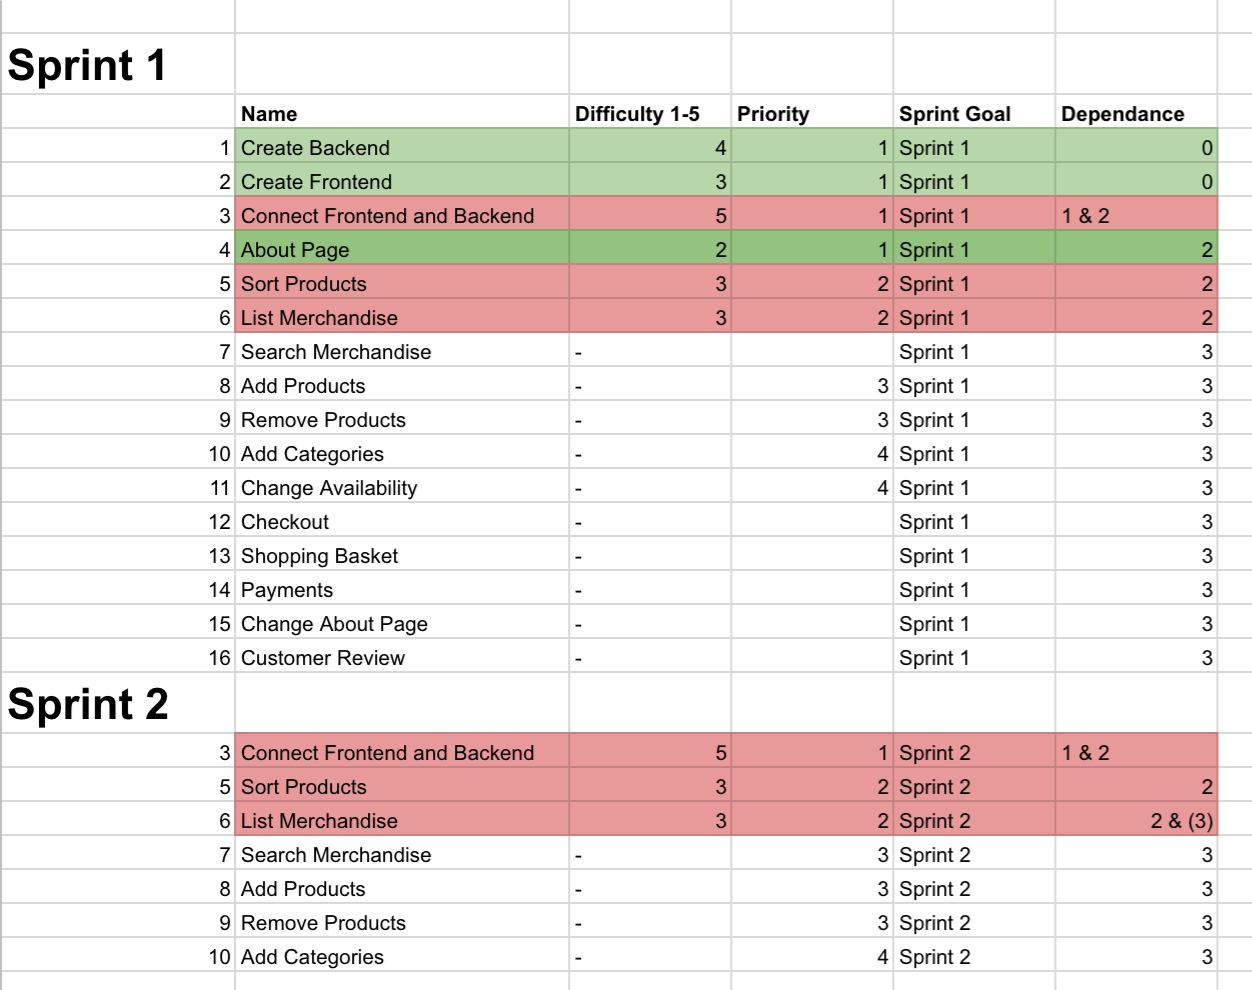
\includegraphics[height=12cm, width=11cm]{sprint1.png}

\newpage
\subsection{Database-Schema}
The database looks as following after sprint 1.
\begin{figure}[H]
    \center
    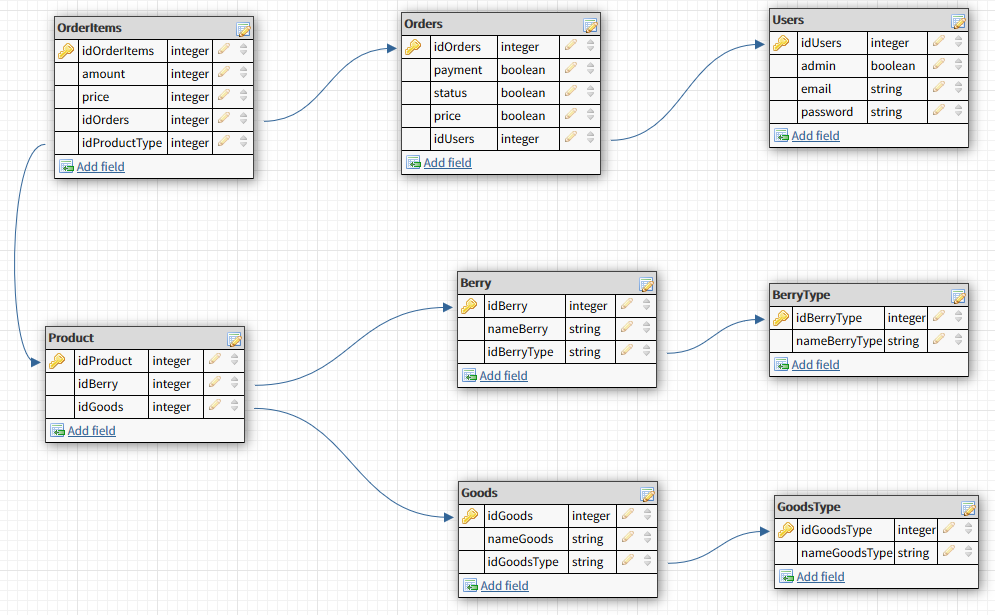
\includegraphics[height=6cm, width=9cm]{new_db_schema.PNG}
\end{figure} 

\textbf{Users:}
Keeps the users with an id, email and password. Also a setting for whether the user is an admin or
not. 
\\
\\
\textbf{Orders:}
Keeps orders with a foreign key idUsers to the id from table Users. Also keeps whether the order is
paid, handled and what the price of the order was. The shopping basket is treated as an order as
well.
\\
\\
\textbf{OrderItems:}
The items of an order with foreign keys idOrders and idProduct to the tables Orders and Product.
Keeps the amount, price and id of a product in an order.
\\
\\
\textbf{Product:}
Foreign keys idBerry and idGoods to the tables Berry and Goods.
\\
\\
\textbf{Berry:}
Foreign key idBerryType to table BerryType. Contains name of berry.
\\
\\
\textbf{Goods:}
Foreign key idGoodsType to table GoodsType. Contains name of goods.
\\
\\
\textbf{BerryType:}
Contains Berry category.
\\
\textbf{GoodsType:}
Contains Goods category.
\newpage
\subsection{Test-cases}

Support for tests was added in the following steps. A test container was added to docker. When that container runs, it performs all the tests using pytest~\cite{pytest}. Code coverage analysis is then reported using coverage.py~\cite{coverage}. 

Support for Selenium~\cite{selenium} was also added, in order to support end-to-end testing. Selenium relies on the browsers Firefox/Google Chrome, and so far attempts to make those run in docker have been unsuccessful. There are hopes, however, that such support will be able to be implemented before long.

Thus, though no actual test cases have been written, the groundwork was laid for being able to perform automated tests.

\newpage